%\part{Introduction}

\chapter{Introduction}

The process of designing electrical circuits consists of several stages, starting with a detailed specification from the customer that provides all necessary requirements, and ending with a working prototype of the final product. Intermediate stages include prototyping circuits using a construction base commonly referred to as a breadboard, which is is often very slow and for complex integrated circuits even impossible. The task has been made easier with the invention of electrical circuit simulation programs, which allow quick circuit prototyping without the need of a soldering iron.

\section{Berkeley SPICE}
One of the most successful circuit simulators is the SPICE program\footnote{The name SPICE stands for Simulation Program with Integrated Circuit Emphasis.} developed at the EECS Department of the University of California, Berkeley. The original SPICE1 program is implemented in the FØRTRAN language and was released in 1971. Its popularity quickly rose and a few years later, Berkeley released SPICE2 with many performance improvements and model enhancements. The SPICE programs developed at Berkeley heavily influenced the development of future circuit simulation software, and we will describe them in more depth in the following sections.

\subsubsection*{Netlists}
Early versions of SPICE did not operate in interactive mode, therefore the input files contained both data and instructions for processing. These input files conventionally have the \texttt{.cir} extension, and the contained circuit description is called a \textit{netlist}. A simple example of netlist is shown on the figure~\ref{fig:example_circuit} on the left, with a schematic of the corresponding circuit on the right. The meaning of individual lines of the netlist is explained in the next paragraph.

\begin{figure}[h]
\centering
\begin{subfigure}{.25\textwidth}
\begin{spicecode}
BRIDGE-T CIRCUIT
*
VBIAS 1 0 12
R1 1 2 10
R2 2 0 10
R3 2 3 5
R4 1 3 5
*
.OP
.END
\end{spicecode}		
	\end{subfigure}\hspace{5mm}
	\begin{subfigure}{.7\textwidth}	
	\centering	
		\begin{circuitdev}
			(0,0) 
			to[V=12<\volt>,invert,a=VBIAS] (3,0) node[label={-90:$1$}]{}
			-- (6,0)
			to[R, l=5<\ohm>, .-*, a=R4] (6,3) node[label={3:$3$}]{}
			to[R, l=5<\ohm>, a=R3] (3,3) node[label={$2$}]{}
			to[R, l=10<\ohm>, a=R2] (0,3)
			-- (0,0)
		
			(3,0) to[R, l=10<\ohm>, a=R1, *-*] (3,3)
			(0,1.5) -- (-0.5,1.5) node[ground]{}
		\end{circuitdev}
\end{subfigure}
	\caption{Example \texttt{.cir} netlist file, reproduced from The SPICE Book \cite{spice_book} and the corresponding circuit schematic}
	\label{fig:example_circuit}
\end{figure}

The netlist in figure~\ref{fig:example_circuit} is divided into three sections, separated by empty comments on lines 2 and 8. The first section of the netlist contains the name of the circuit, then follows a second section with definitions of five devices: one voltage source and four resistors. The type of each device is inferred from the first letter of its name. Each definition contains a list of connected nodes and the value of a source voltage or a resistor's ohmic resistance, respectively. Node 0 is special, because it corresponds to the ground and must be present in every circuit (a detailed description of SPICE netlists syntax and rules for validating the circuit will be presented later in chapter~\ref{chap:spicecode}). In the last section of the file, there is an \texttt{.OP} statement, which instructs the simulator to perform an operating point analysis to find stable values of node voltages of the circuit, and an \texttt{.END} statement denoting the end of the netlist. This syntax for describing electrical circuits became an industry standard during the 1970s, and most modern circuit simulators still recognize it.

When SPICE2 is run with the previously shown netlist file, it first reads all components, checks syntax and topology rules for the circuit, and then runs the operating point analysis -- computes node voltages and current through the \texttt{VBIAS} voltage source. After that, it prints a rather verbose report, as shown in figure~\ref{fig:example_output}. First, a description of the input circuit is repeated back to the user (only part of the description is shown in the figure for brevity, in the top half in grey), then follows a list of node voltages and then currents flowing through voltage sources.

\begin{figure}[h]
	\begin{spicecode}
\color{lightgray}******* 03/19/91 ********* SPICE 2G.6  9/21/84 ********* 06:47:36 *********
	
\color{lightgray}BRIDGE-T CIRCUIT
	
\color{lightgray} ****     CIRCUIT DESCRIPTION

\color{lightgray}***************************************************************************
\color{lightgray}*
\color{lightgray}VBIAS 1 0 12
\color{lightgray}...
\color{lightgray}.END

******* 03/19/91 ********* SPICE 2G.6  9/21/84 ********* 06:47:36 *********

BRIDGE-T CIRCUIT

 ****  SMALL SIGNAL BIAS SOLUTION   TEMPERATURE = 27.000 DEG C
 
***************************************************************************

 NODE    VOLTAGE     NODE    VOLTAGE     NODE    VOLTAGE    NODE   VOLTAGE

(    1)    12.0000  (    2)     8.0000  (    3)    10.0000 

    VOLTAGE SOURCE CURRENTS
    NAME         CURRENT
    
    VBIAS       -8.000E-01
    
    TOTAL POWER DISSIPATION 9.60E+00 WATTS
	\end{spicecode}
	\caption{Output of SPICE2G.6 for the example netlist file, from The SPICE Book \cite{spice_book}}
	\label{fig:example_output}
\end{figure}


\subsubsection*{Macromodels}
One of the most useful features of SPICE is the ability to define custom subcircuits, called \textit{macromodels}, composed from devices already integrated in the simulator, or other macromodels. Circuits can be then decomposed into individual subcircuits, similarly to how a computer program's source code can be decomposed into individual functions. One macromodel can then represent a complex real-life device, e.g. an amplifier, and can be simply reused throughout the whole circuit.

This allows device manufacturers to provide SPICE netlists with macromodels that accurately model their devices. An example of such a manufacturer is Analog Devices, macromodels for their products can be downloaded from their webpage, a screenshot of which is shown in figure~\ref{fig:analog-macromodel-website}. The manufacturer's customers can then use these macromodels in their simulators to model the behavior of a circuit that uses the manufacturer's products.

\begin{figure}[h]
	\centering
	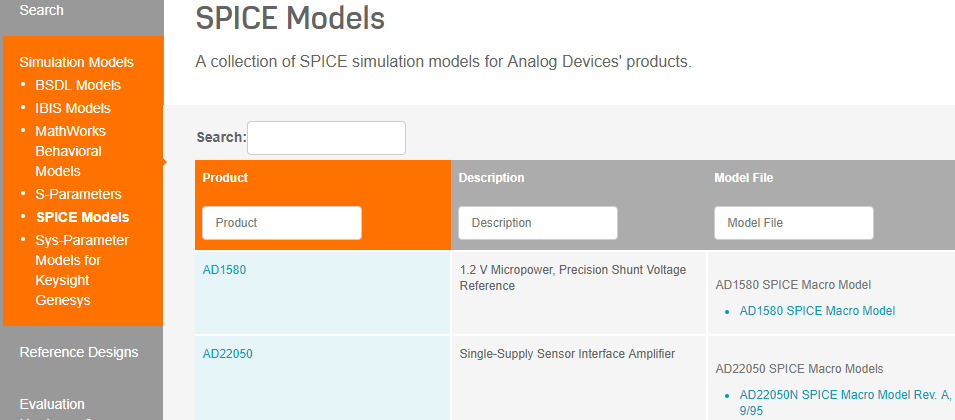
\includegraphics[width=\textwidth]{01-fig-analog-website-macromodels.png}
	\caption{Website of Analog Devices, where SPICE macromodels can be downloaded.}
	\label{fig:analog-macromodel-website}
\end{figure}

Today, vast libraries containing hundreds of SPICE netlists with macromodels exist, and therefore it is a very important feature of any modern circuit simulator to be able to import macromodels from these netlists.

Manufacturer-supplied macromodels are often very complex and the netlists are too long to be shown here. Instead, the use of macromodels is demonstrated on a simple macromodel for an AC coupled amplifier. The netlist description is shown in figure~\ref{fig:example_subcircuit}. A very important part of the definition is the opening \texttt{.SUBCKT} statement, which denotes the start of the subcircuit description, and specifies its name and terminal nodes which will serve as an interface to the outer circuit. After that follows a description of the devices that constitute the macromodel, and finally, the subcircuit definition is ended by an \texttt{.ENDS} statement. The subcircuit in the figure is named ACamplifier and the terminal nodes are 1, 2 and 3. Other nodes (excluding \texttt{0}, which is a global ground node) and all devices used between the \texttt{.SUBCKT} and \texttt{.ENDS} statement are strictly local to the subcircuit and are not visible to the outside circuit.

\begin{figure}[H]
	\centering	
	\begin{subfigure}{.43\textwidth}
	\begin{spicecode}
* external nodes:  in power out
.SUBCKT  ACamplifier 2 1 3
R1 1 4 2K
R2 4 0 500
C1 2 4 10n
Q1 3 4 5 2N2222
Rc 1 3 2K
Re 5 0 1e3
.MODEL 2N2222 NPN 
+ (BF=50 IS=1E-13 VBF=50)
.ENDS
	\end{spicecode}		
\end{subfigure}\hspace{5mm}
\begin{subfigure}{.5\textwidth}	
	\begin{circuitdev}
		(0.3,0) node[circ,label=1]{}
		-- (5.5,0)
		to[R=Rc, a=2<\kilo\ohm>] (5.5,-2)		
		node[npn, label={right:Q1 2N3904}, anchor=C](npn) {}		
		(npn.emitter) node[label=1:5]{}
		to[R=Re, a=1<\milli\ohm>, *-] (5.5, -6) node[ground]{}
		-- (2.5, -6)
		to[R=500<\ohm>, a=R2] (2.5, -3.3)
		-- (2.5,-2.93) node[label=3:4]{}
		-- (npn.base)
		-- (2.5,-2.93) 
		to[R=2<\kilo\ohm>, a=R1] (2.5,0)
		(2.5,-2.93) to[C=10<\nano\farad>, a=C1, *-*]
		(0.3, -2.93) node[label=2]{}
		
		(5.5, -2) -- (6.6,-2) node[circ,label=3]{}
	\end{circuitdev}
\end{subfigure}
\caption{Simple macromodel example for AC coupled amplifier \cite{5spice-subcircuit}, and corresponding circuit schematic, adapted from a 5Spice tutorial by Richard P. Andresen}
\label{fig:example_subcircuit}	
\end{figure}

Such a macromodel can then be used by providing nodes for terminal connections. In a SPICE netlist, a macromodel is represented by a device with a name staring with an X. The actual macromodel to be used is specified as the last argument in the device statement. An example of a circuit that uses the ACamplifier macromodel is shown in figure~\ref{fig:example_subcircuit_call}. The macromodel definition is inlcuded from a separate file, similarly to the \texttt{\#include} preprocessor directive in C or C++. In the actual circuit, the macromodel is represented by the \texttt{XAMP} device. Nodes 3, 2 and 1 are mapped onto the nodes 2, 1 and 3 from the macromodel description.

\begin{figure}[h]
	\centering	
	\begin{subfigure}{.35\textwidth}
		\begin{spicecode}
SUBCIRCUIT CALL EXAMPLE
*
.INCLUDE acamplifier.cir
*
V1 2 0 5
R1 2 3 10
XAMP 3 2 1 ACamplifier
R2 3 0 20
*
.END
		\end{spicecode}		
	\end{subfigure}\hspace{1mm}
	\begin{subfigure}{.61\textwidth}	
		\begin{circuitdev}
			
			(-1,0) to[R=10<\ohm>, a=R1, *-*] (-1, -2.93)
			
			(-2.5,-8.5) to[V=5<\volt>, a=V1, invert]			
			(-2.5,0) -- (-1, 0) node[label={$2 = 1'$}]{}
			-- (4.5,0)
			to[R] (4.5,-2)		
			node[npn, anchor=C](npn) {}		
			(npn.emitter) 
			to[R] (4.5, -6) node[ground]{}
			-- (2.5, -6)
			to[R] (2.5, -3.3)
			-- (2.5,-2.93) 
			-- (npn.base)
			-- (2.5,-2.93)
			to[R] (2.5,0)
			(2.5,-2.93) to[C] (0, -2.93)--
			(-1, -2.93) node[label=270:{$3 = 2'$}]{}
			
			(4.5, -2) -- (6.3,-2) node[circ,label=90:{$1 = 3'$}]{}
			-- (6.3, -8.5) to[R=20<\ohm>, a=R2] (-2.5,-8.5) node[ground]{}	
			;
			\draw[draw=black, very thick, fill=lightgray, fill opacity=0.8] (0.5,0.5) rectangle ++(5,-7.7) ;
			\node at (3,1) {XAMP (ACamplifier)}
		\end{circuitdev}
	\end{subfigure}
	\caption{Illustrative example of circuit that uses macromodel from figure~\ref{fig:example_subcircuit}}
	\label{fig:example_subcircuit_call}	
\end{figure}

\subsubsection*{From SPICE2 to SPICE3}
SPICE2 was not the last SPICE program developed at Berkeley. With the increasingly more popular UNIX-based operating systems, it was possible for programs to be more interactive. Andrei Vladimirescu states in The SPICE Book \cite{spice_book} that SPICE2 was \shortquote{a FORTRAN batch program and was difficult to modify and limited in its potential use of C-shell utilities}. These limitations led Berkeley to start the development of SPICE3 in the C programming language during the 1980s. In addition to more detailed models and improved numerical accuracy, SPICE3 was to support interactive mode, which allowed separating the circuit description from commands for requesting circuit analysis.

Unfortunately, the development was in the end left to a handful of students due to limited financial resources. The first release of SPICE3 was very buggy and was not backward compatible with SPICE2. This was a big problem, because hundreds of commonly used macro-models would have to be rewritten before they could be used in SPICE3. Even though most incompatibility issues were fixed in later releases, SPICE3 did not completely replace SPICE2 and both coexist as two standards for circuit simulations, with the SPICE2 one being a subset of SPICE3 and therefore more portable.

\section{Present-day Situation}
The SPICE programs developed at Berkeley strongly influenced the development of circuit simulators used in industry. Because of the vast existing libraries of SPICE netlist files for various circuits, most circuit simulators either use a syntax which is a superset of the one used in SPICE, or provide some other way of importing circuits from the standard SPICE format.\footnote{Example of a simulator which does not support SPICE syntax directly is QUCS simulator, which provides a tool for transforming the netlist in SPICE format into the QUCS format.} There is even a categorization of circuit simulators based on their backward compatibility with Berkeley SPICE programs. Ron Kielkowski summarizes this in Inside SPICE \cite{inside_spice} as follows:

\begin{blockquote}
	Of all the analog circuit simulation tools available, the overwhelming majority of them are SPICE-like or SPICE-compatible. SPICE-like means a simulator is capable of producing an analysis result similar to the SPICE result for a given circuit, although they many not be able to read a standard SPICE circuit. SPICE-compatible means a simulator can read a SPICE circuit file and produce the result in standard SPICE2G.6 form.\footnote{Result shown in figure~\ref{fig:example_output} is an example of such standardized output.}
\end{blockquote}

This only reinforces the idea that backward compatibility with the original SPICE programs is an important feature of circuit simulators.

Today's circuit simulating programs commonly include a graphical tool for editing circuits and plotting the simulation results. Instead of writing netlist files by hand, circuits are edited using drag-and-drop operations. One such program is LTspice \cite{ltspice-web}, whose graphical user interface is shown in figure~\ref{fig:ltspice-gui}.

\begin{figure}[h]
	\centering
	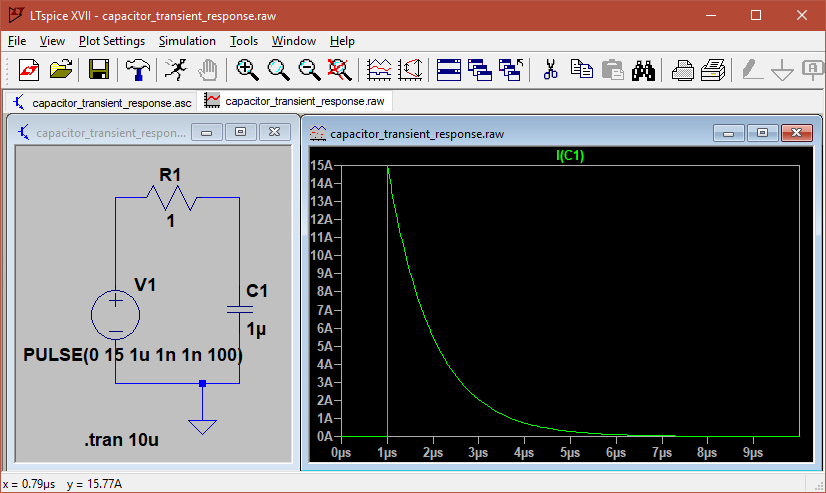
\includegraphics[width=\linewidth]{01-fig-ltspice.png}
	\caption{Graphical user interface of LTspice}
	\label{fig:ltspice-gui}
\end{figure}

\section{Use of Circuit Simulators Outside Industry}
The Berkeley SPICE programs were designed from the start to be used as an aid for integrated circuit designers. The same can be said about SPICE's successors that are used today. However, thanks to a significant increase in computational power, it is now possible to use circuit simulators in other contexts too. There is ongoing research on the use of evolutionary algorithms to evolve circuit parameters and even circuit topology. For example, in 2016, Rojec et al.\ successfully evolved a passive low-pass filter \cite{Rojec2016}. Also, computers and other interactive equipment are often used for educational purposes in schools, so a circuit simulator can be used as part of an educational program intended for high school or university students.

We have in mind creating such applications, and their development would be greatly simplified if there was a suitable circuit simulation library. We would essentially like the simulator to allow what we will call a \textit{live simulation}. For example, in a potential educational program, we would like to allow the user (a student) to e.g.\ flip switches or manipulate parameters of individual devices (e.g.\ resistances on the resistors), and hence provide an interactive experience. Also, circuit evolution applications could also make use of the possibility to simply manipulate circuit parameters. The first step of development of these applications would be finding and preparing such a simulation library.

Since such applications would be used primarily for academic or educational purposes, it is desired that these programs be easy to develop, maintain, and -- in the case of educational applications -- support multiple platforms. For these reasons it is probable that these applications would not be developed in some low level language like C++, but rather a higher level language. One such language, C\#, is part of the .NET developer platform, which is widely used in desktop application development. In recent years, .NET has expanded to other platforms as well and would be therefore our choice for the development of said applications.

As we have written earlier, SPICE programs and their descendants were designed mainly to be an aid for electrical engineers. As a consequence, they can only perform off-line simulation, where the simulated period needs to be set explicitly before the simulation starts. During our research we did not find any simulator which would allow the simulation to be continued where it left off.\footnote{For simple circuits, this can be achieved by setting the initial conditions of the circuit devices to be equal to the state of the circuit at the end of previous simulation, and recomputing the parameters for input sources (like phase offset and pulse delay). However, it is impossible to get or let alone set state of a device inside a subcircuit (the X device).} Furthermore, most simulators do not offer a binary API for other programs to use, which means that the communication with the simulator needs to be done through the SPICE netlist files. One simulator which stands out is ngspice \cite{ngspice}, which exposes a set of functions that allow manipulation of the simulator from an external program. The ngspice API does not require the input file to be written on disk, but we are still required to convert a simulated circuit into a netlist description, which is then passed to ngspice using a \texttt{char**} pointer.\footnote{For more details, see section 19.3 (Shared ngspice API) in ngspice user manual \cite{ngspice-manual}.}

Existing simulator programs therefore are not suitable for our purpose, we should search among the existing simulator libraries. At the time of assignment of this thesis, there was no implementation of a circuit simulation library for the .NET Framework.\footnote{At the time of writing, there is the SpiceSharp \cite{spicesharp} library, whose development started shortly after that of NextGen SPICE.} There are libraries for Python, for example PySpice \cite{pyspice} and PyOPUS \cite{pyopus} -- but these two libraries rely on standalone simulators (namely ngspice \cite{ngspice} and HSPICE \cite{hspice}) to do the simulation and therefore share the same limitations. There is also the JSpice \cite{jspice} library for Java, which implements it's own simulation engine, but just like other simulators requires the user to specify a simulation duration beforehand.

A possible solution to the problems of using present-date simulator programs or libraries is rewriting an existing circuit simulator in the .NET Framework and making necessary changes to the interface for our purpose. Berkley SPICE3 is still considered a reference simulator program, and since it is open source and freely available on the website of University of California, Berkeley \cite{spice3f5}, we will examine the possibility of rewriting it in .NET in the next subsection.

\subsubsection*{Rewriting SPICE3 for .NET, a Viable Option?}

SPICE3 was written in now non-standard K\&R C, because the development started years before the first ANSI norm was released in 1990. Due to the nature of the C language, many parts of the simulator are very fragile and hard to maintain from today's perspective. Consider the snippet in figure~\ref{fig:vccs_snippet} taken from the last SPICE3 release (version 3f.5 from 1993). It contains a function which loads instances of voltage controlled current source devices to a circuit equation matrix. This function is just one example from the set of functions that must exist for each device in the SPICE3 implementation. Other such functions include methods for model updating and data printing.

\begin{figure}[h]
	\begin{minted}[linenos, tabsize=4]{cpp}
/*ARGSUSED*/
int
VCCSload(inModel,ckt)
	GENmodel *inModel;
	CKTcircuit *ckt;
		/* actually load the current values into the 
		 * sparse matrix previously provided 
		 */
{
	register VCCSmodel *model = (VCCSmodel *)inModel;
	register VCCSinstance *here;
	
	/*  loop through all the source models */
	for( ; model != NULL; model = model->VCCSnextModel ) {
		
		/* loop through all the instances of the model */
		for (here = model->VCCSinstances; here != NULL ;
		here=here->VCCSnextInstance) {
			
			*(here->VCCSposContPosptr) += here->VCCScoeff ;
			*(here->VCCSposContNegptr) -= here->VCCScoeff ;
			*(here->VCCSnegContPosptr) -= here->VCCScoeff ;
			*(here->VCCSnegContNegptr) += here->VCCScoeff ;
		}
	}
	return(OK);
}
	\end{minted}
	\caption{Code snippet from \texttt{spice3f5/src/lib/dev/vccs/vccsload.c}}
	\label{fig:vccs_snippet}
\end{figure}

There are many points worth mentioning. In the declaration of the \texttt{VCCSload} function, the function parameters are specified by name only (line 3). The type of each parameter is then specified separately (lines 4--5). This is the main characteristic of K\&R C. In ANSI C, the equivalent declaration would be \texttt{VCCSload(GENmodel *inModel, CKTcircuit *ckt)}.

The next thing to notice is the pointer casting on line 10 -- the \texttt{inModel} parameter is cast to a pointer to the concrete type of the device that is being loaded. Practices like this are very common in C code due to the lack of higher-level language features like inheritance and polymorphism. Also, because no type checking occurs in C during pointer casting, it can be a source of hard-to-debug errors if the target object is of a different type.

Lines 10 and 11 also include the \texttt{register} keyword, which used to be a hint for the compiler to store the variable in a CPU register for faster access. This keyword is now deprecated, because modern compilers can do a better job at assigning variables to registers than a human programmer.

The last point worth noticing is the usage of pointers when accessing the equation matrix (lines 20 to 23). C\# does allow the usage of pointers in a so called \textit{unsafe code block}, but they affect the performance of the garbage collector, and should be used carefully.

Although it is possible to extend SPICE3 with new circuit devices by following instructions from Thomas Quarles, the author of SPICE3 \cite{Quarles:M89/45}, adding new analysis types requires modifying method tables for all existing devices and other crucial parts of the simulator, and thus is time consuming and error-prone.

The SPICE3 code also makes heavy use of \texttt{\#define} \texttt{\#ifdef} and other preprocessor directives which make the source code less readable. In combination with long functions and scarce source code documentation available (for an example, see file \texttt{spice3f5/src/lib/ckt/dctran.c}), rewriting the simulator is a very hard task requiring in-depth analysis and understanding of the simulator internals.

Overall, the programming style used in the SPICE3 implementation is very different from the style used in modern object oriented programming languages like C\#, and its code is not suitable for simple one-to-one translation from C to C\#.

\subsubsection*{Main thesis goal}
Because of the reasons listed so far in this chapter, computer programs which would as part of their functionality perform live simulation of electrical circuits would have to implement their own simulator engine. As the primary goal of this thesis, we would like to simplify the development of such applications by implementing such a circuit simulator from the ground up in the form of a portable .NET library. We will specify our requirements for the library in the next section.

\section{Reimplementation of SPICE for .NET}

Modern circuit simulators can do many types of circuit analyses and support many types of circuit devices. Because implementing a range of functionality comparable to these programs would be out of scope of this thesis, we have selected a reasonable subset to be implemented, which is described in the following subsection in greater detail. However we would like to be able to implement other features in the future without affecting the user's code. We would therefore have to design the library to be appropriately extensible.

\subsubsection*{Requirements on the Library}

We would like the library to be usable in broad contexts. Since .NET is now supported on many platforms, including Windows, Linux, and even mobile devices (Android, iOS and Windows Mobile), the library should be targeted to .NET Standard to make it maximally portable and usable on any .NET platform.

Our primary goal in the library will be supporting live simulation, as we described earlier. This essentially requires implementing the equivalent of \textit{transient analysis} of the SPICE simulator. However, the simulator should perform the individual timesteps on demand and allow making reasonable changes to the circuit devices like flipping switches, changing resistances, changing values of voltage and current sources.

Transient analysis requires so called \textit{large-signal} models of the simulated devices, which are also used by other types of SPICE-like analyses, like DC Sweep Analysis. DC Sweep analysis calculates the circuit states for a range of values for a certain circuit parameter (like the resistance of a resistor or the value of a voltage/current source). Because we already wish to support changing parameters between individual timesteps, our library will also support DC Sweep analysis.

We would like to design our library so that it could potentially support the same set of devices as the SPICE simulators. However, the implementation of all SPICE devices is quite complex and would be out of scope of this thesis. We have therefore decided to implement basic devices like ideal resistors, voltage or current sources, capacitors and inductors. Also, to demonstrate that even complex semiconductor devices can be implemented, we will implement diode and BJT transistor devices as well. These two devices are reasonably simple to implement and at the same time complex enough to demonstrate the capabilities of the simulator. Because SPICE is considered the reference circuit simulator implementation, we would implement these devices using the same mathematical models that are used in the SPICE simulators.

In the future, we would also like to add other types of circuit analyses -- such as AC frequency sweep analysis -- and new devices, and even allow users of our library to implement their own. The library should be therefore extensible without modifying the core library's source code. 

To provide academic researchers with a way to test newly developed models and computational techniques, the library should be widely configurable, and preferably open-source, to allow its users to contribute to the library's development.

Also, since there already exist vast libraries of spice circuits and subcircuits with macromodels described in the industry-standard SPICE netlist syntax, we would like to our library to support importing circuits from SPICE netlists. We will therefore provide a SPICE netlist parser as part of our library.

Since we have to recognize great portion of the SPICE netlist syntax in order to parse macromodel descriptions, with little additional work we could implement a parser to recognize control statements for requesting individual circuit analyses (like the \texttt{.OP} statement we saw in figure~\ref{fig:example_circuit}). This would allow us to create a console application similar to the original SPICE and therefore allow capabilities of the library to be used in a standalone fashion using the SPICE netlist syntax. Since .NET Standard cannot be used to develop console applications, we require that the console application requires the next smallest set of API: .NET Core. Figure~\ref{fig:deps} shows the expected relationship between the simulator, console application and other programs that would use the simulator -- parts in blue will be implemented as part of this thesis.

\begin{figure}[h]
	\centering
	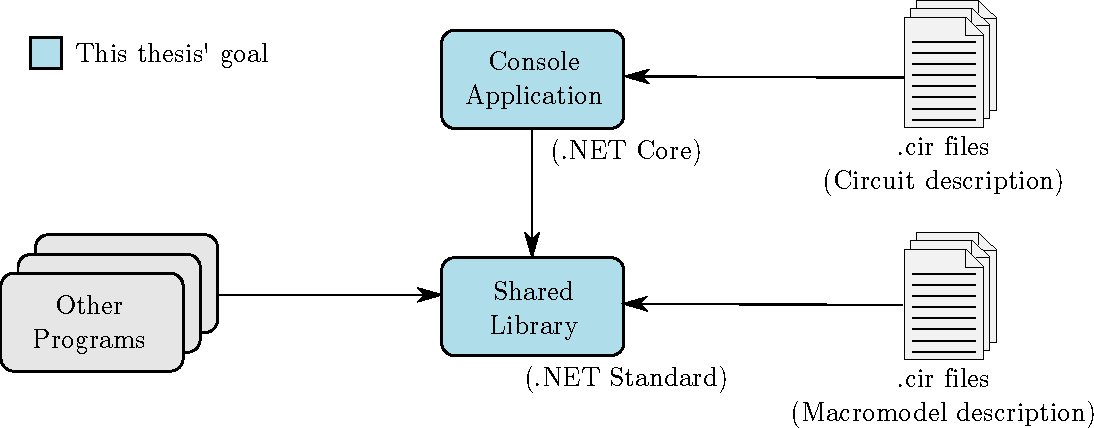
\includegraphics[width=0.8\linewidth]{deps-intro}
	\caption{Dependency diagram for NextGen SPICE and other programs}
	\label{fig:deps}
\end{figure}


\subsubsection*{Nonconvergence Due to Low Precision}
\label{chap:intro:dd}
Implementing any kind of simulation software means choosing an appropriate mathematical model for the given problem domain and, subsequently, a suitable representation of the problem in computer memory. Representing real numbers is an integral part of every physics simulation engine.

To achieve fast simulations, developers have to choose between representations having hardware support on the target platforms, which leaves them with IEEE 32-bit (\texttt{single}) and 64-bit (\texttt{double}) floating-point types. 

Most of the common circuit simulators use type \texttt{double} with approximately 15 decimal digits of precision. Due to the large dynamic range of the circuit variables, this leads to significant truncation errors when equation system coefficients differ in more than 15 orders of magnitude.

Coefficient differences of this magnitude may commonly occur when resistors with very small resistance values are used. Mike Robbins, one of the authors of the online circuit simulator CircuitLab, provides a simple example of such an ill-conditioned circuit in an article on their website \cite{circuitlab_dd}. This circuit along with the (partial) result plot from LTspice can be found in the upper part of figure~\ref{fig:ltspice-precision}. Notice the noise at the end of the simulated period emphasized by the red arrow. The lower part contains result of the same circuit in the CircuitLab simulator.\footnote{Keen reader might notice differences between the plot of CircuitLabs simulator results shown in this thesis and the one in the referenced article. These are due to the fact that CircuitLab uses slightly different model parameters for 1N4148 diode than LTspice. Plot shown in this thesis was obtained using the model parameters extracted from LTspice model library.}

\begin{figure}[h]
	\centering
	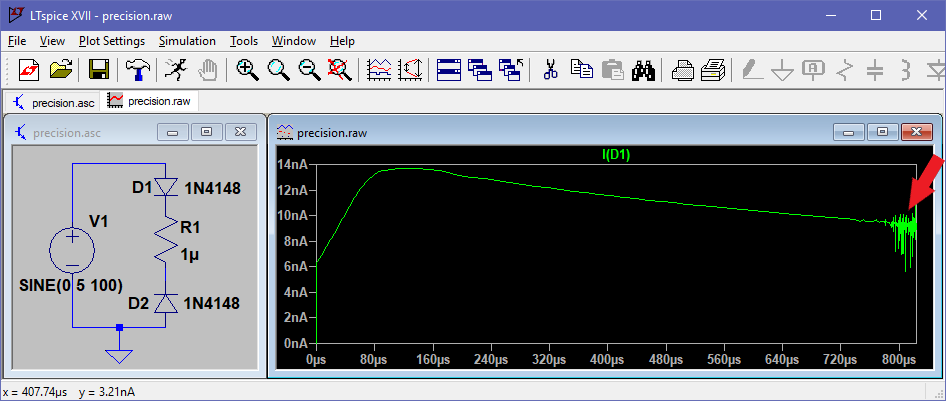
\includegraphics[width=0.8\textwidth]{01-fig-ltspice-precision}
	\caption*{LTspice}
	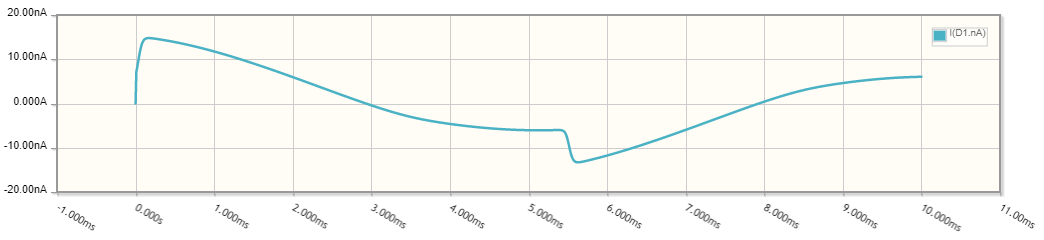
\includegraphics[width=0.8\textwidth]{01-fig-ltspice-precision2}
	\caption*{CircuitLab}
	\caption{Example ill-conditioned circuit, and example results form LTspice (top, incomplete), and CircuitLab (bottom), adapted from \cite{circuitlab_dd}}
	\label{fig:ltspice-precision}
\end{figure}

The noise in the plot on the figure is caused by the $1\mu\Omega$ resistor in the circuit. In the comment section under the article, Robbins writes that such small resistors are not physical, meaning that they do not correspond to physical resistor devices, but can be produced during automated macromodel construction. Use of this small resistor led to too-big differences between the equation coefficients, which in turn led to significant truncation errors and produced noise seen in the plot. This noise later leads to nonconvergence of the equation solution. Nonconvergence of the solution is a rather technical issue, and essentially means that the simulator cannot determine the state of the circuit after the next timestep.\footnote{In general, there are many reasons why solution might not converge, several possible techniques and simulator parameters used to overcome nonconvergence are explained in Ron Kielkowski's Inside SPICE \cite{inside_spice}.} In this case, the nonconvergence is caused by low precision of the representation of real numbers.

Such noise can be eliminated by using a more precise real number representation. One such option is using another type defined by the IEEE 754 standard, namely 80-bit or even 128-bit floating point number formats. However, neither of these is commonly available on today's hardware, let alone in the .NET runtime. If we would decide to use one of these two formats, every operation on such numbers would have to be emulated in software, which would greatly slow down the simulator.

Another option would be using the .NET type \texttt{decimal} which is a 128-bit representation of floating point numbers different from the IEEE 128-bit format. Its format is not directly supported on currently used processors, and therefore all operations are implemented in software by bit manipulations. Also, this type is intended mainly for handling currency and has an approximate range of only $-7.9 \cdot 10^{28}$ to $7.9 \cdot 10^{28}$,  which is too-narrow for circuit simulation.

Instead, in the article mentioned above, Mike Robbins proposes using the double-double technique. This technique represents a single value as a unevaluated sum of two \texttt{double} floating point values, each of which has its own significand and exponent. This principle is illustrated in figure~\ref{fig:dd_pi} where number $\pi$ is represented as a sum of two doubles.\footnote{One thing worth noting is that an implementation of the double-double format needs to decompose values based on the the binary representation of the real numbers. The QD library by Hida et al.\ \cite{qd-lib} uses values 3.141592653589793116e+00 and 1.224646799147353207e-16 in the source code, possibly to compensate errors from truncating periodic binary representation of the mantissa.}

\begin{figure}[h]
	\centering	
$\underbrace{3.141592653589793}_{ }\underbrace{238462643383279}$ 

$3.141592653589793 \cdot 10^{0} + 2.38462643383279 \cdot 10^{-16}$

	\caption{Decomposition of $\pi{}$ using double-double technique}
	\label{fig:dd_pi}
\end{figure}

Contrary to the options mentioned above, operations on the double-double format are implemented using standard operations on the \texttt{double} format, which are supported in today's hardware. This means that much higher speeds can be achieved. Hida et al.\ created a C++ library, that implements both double-double arithmetic, and it's slightly more complicated version -- quad-double arithmetic. More details about the algorithms used can be found in their published paper \cite{Hida2007}. 

Using these enhanced precision types is attractive, because they can solve some convergence issues during simulation, and we would therefore like to use them in our library. However, use of these precision types could lead to significant slowdown of the simulation, because multiple primitive operations on \texttt{double}s are done for each operation on the double-double and quad-double types. This could unnecessarily slow down simulations of circuits which do not require the precision provided by these types. We would therefore like to make these enhanced precision types optional, and otherwise use the standard \texttt{double} precision type. Because our implementation will allow using any of the \texttt{double}, double-double and quad-double types, we would like to compare the simulator performance -- i.e.\ speed and accuracy -- when using each of these types to get the basic idea when use of these types is appropriate.

\section{Goals}
\label{chap:intro:goals}

\begin{enumerate}
	\item Implement a SPICE-like simulation library	
	\begin{enumerate}
		\item Target .NET Standard for maximum portability
		\item \label{goal:transient} Support performing time-domain simulation of the circuit, and allow changing parameters of circuit devices between individual timesteps.
		
		\item \label{goal:devices} Support the following set of devices
		\begin{enumerate}
			\item Ideal resistor
			\item Ideal voltage source
			\item Ideal current source
			\item Ideal inductor
			\item Ideal capacitor
			\item SPICE diode
			\item SPICE BJT transistor
		\end{enumerate}
	
		\item \label{goal:extension} Allow new types of circuit analyses and circuit devices to be added to the simulator without modifying the library's source code.
	
		\item \label{goal:parser} Implement a SPICE netlist parser to allow importing circuits and macromodels from standard SPICE netlist files.

		\item \label{goal:dd} Allow users of the library to choose between double, double-double, and quad-double precision types and compare the library's performance with respect to speed and accuracy for each listed precision type.
	\end{enumerate}

	\item \label{goal:app} Use the simulation library to implement a SPICE-like console application for .NET Core, which would accept the implemented subset of SPICE netlist syntax.
\end{enumerate}
